\documentclass[sigconf,review=false,anonymous=true]{acmart}
\acmConference[]{Conference}{Venue}{Date}

\usepackage{balance}
\usepackage{booktabs} % For formal tables
\usepackage{csquotes}
%\usepackage{graphicx}
\usepackage{enumitem}
\usepackage{blindtext}
\usepackage{lipsum}

\setlength{\fboxsep}{4pt}

% remove next three lines for CRC
\settopmatter{printacmref=false} % Removes citation information below abstract
\renewcommand\footnotetextcopyrightpermission[1]{} % removes footnote with conference information in first column
\pagestyle{plain} % removes running headers

\newtheorem{ra}{Answer}
\newtheorem{obs}{Observation}
\newtheorem{req}{\textbf{RQ}}
\newtheorem*{obsUnNum}{Observation}

\newcommand{\papertitleA}{Semantic Source Code History}
\newcommand{\papertitle}{\papertitleA}

\newcommand{\todo}[1]{\textbf{\color{red}#1}}
\newcommand{\commentout}[1]{}

\newcommand{\mybox}[1]{\vspace{5pt}\noindent\fbox{\parbox{0.97\columnwidth}{#1}}\vspace{5pt}}


% from: https://tex.stackexchange.com/a/62171
\usepackage{tikz}
\usetikzlibrary{shapes,fit,backgrounds}
\usepackage{xifthen}

% Hyperref
\usepackage{hyperref}
\hypersetup{
   pdfborder={0 0 0},
   pdftitle={\papertitle},
   pdfauthor={},
   pdfsubject={},
   pdfkeywords={},
   pdfproducer={},
   pdfcreator={},
   colorlinks=true,
   citecolor=black,
   filecolor=black,
   linkcolor=black,
   urlcolor=black
}

\usepackage{ifthen}
\usepackage{url}

%\usepackage{changebar} --> does not work with table*
\usepackage{colortbl}
\usepackage{xspace}
\usepackage{xcolor}
\usepackage{tabularx}
\usepackage{color}
\usepackage{txfonts}

\usepackage{listings}
\colorlet{punct}{red!60!black}
\definecolor{background}{HTML}{EEEEEE}
\definecolor{delim}{RGB}{20,105,176}
\colorlet{numb}{magenta!60!black}

\lstdefinelanguage{json}{
    basicstyle=\normalfont\ttfamily,
    numbers=left,
    numberstyle=\scriptsize,
    stepnumber=1,
    numbersep=8pt,
    showstringspaces=false,
    breaklines=true,
    frame=lines,
    backgroundcolor=\color{background},
    literate=
     *{0}{{{\color{numb}0}}}{1}
      {1}{{{\color{numb}1}}}{1}
      {2}{{{\color{numb}2}}}{1}
      {3}{{{\color{numb}3}}}{1}
      {4}{{{\color{numb}4}}}{1}
      {5}{{{\color{numb}5}}}{1}
      {6}{{{\color{numb}6}}}{1}
      {7}{{{\color{numb}7}}}{1}
      {8}{{{\color{numb}8}}}{1}
      {9}{{{\color{numb}9}}}{1}
      {:}{{{\color{punct}{:}}}}{1}
      {,}{{{\color{punct}{,}}}}{1}
      {\{}{{{\color{delim}{\{}}}}{1}
      {\}}{{{\color{delim}{\}}}}}{1}
      {[}{{{\color{delim}{[}}}}{1}
      {]}{{{\color{delim}{]}}}}{1},
}


% Copyright
\setcopyright{none}
%\setcopyright{acmcopyright}
%\setcopyright{acmlicensed}
%%%\setcopyright{rightsretained}
%\setcopyright{usgov}
%\setcopyright{usgovmixed}
%\setcopyright{cagov}
%\setcopyright{cagovmixed}


\newcommand{\tikzmark}[1]{\tikz[overlay,remember picture] \node (#1) {};}

\newcommand{\bubble}[6]% name, content, color, align, inner sep, width
{   \ifthenelse{\equal{r}{#4}\OR\equal{c}{#4}}{\hfill}{}
    \begin{tikzpicture}
        \node[text width=\the\textwidth*#6, below right](#1){#2};
        \begin{pgfonlayer}{background}
            \node[fit=(#1),inner sep=#5,rectangle callout,rounded corners=3pt,draw,fill=#3,overlay] {};
        \end{pgfonlayer}
    \end{tikzpicture}
    \ifthenelse{\equal{l}{#4}\OR\equal{c}{#4}}{\hfill\phantom{}\\[5mm]}{\\[5mm]}
}


% for commenting and making it visible in the pdf (easy to hide after)
\newboolean{hidecomments}
\setboolean{hidecomments}{false}
%\nochangebars
\ifthenelse{\boolean{hidecomments}}
{\newcommand{\cb}[2]{}}
{\newcommand{\cb}[2]{
    \fbox{\bfseries\sffamily\scriptsize#1}
    {\sf\small$\blacktriangleright$ %$\RHD$
      {#2} $\blacktriangleleft$}}} %\LHD$}}}%
\newcommand\fg[1]{\cb{FG}{\textcolor{red}{#1}}}
\newcommand\rth[1]{\cb{RH}{\textcolor{green}{#1}}}

\newcommand{\inlquo}[1]{``\textit{#1}''}
\newcommand{\inlquoP}[2]{``\textit{#1}'' \textit{(#2)}}
\newcommand{\quo}[2]{\\[0.1cm]\noindent ``\textit{#1}'' \textit{(#2)}\vspace*{0.1cm}}
\newcommand{\quoWSp}[2]{\noindent ``\textit{#1}'' \textit{(#2)}}

% DOI
\acmDOI{}

% ISBN
\acmISBN{}

%Conference
%\acmConference[ICSE'18]{40th International Conference on Software Engineering}{May 2018}{Gothenburg, Sweden}
%\acmYear{2018}
%\copyrightyear{2018}
%\acmPrice{15.00}

\begin{document}
\title{\papertitle}

\author{Felix Grund}
\affiliation{%
  \department{Department of Computer Science}
  \institution{University of British Columbia}
  \city{Vancouver}
  \state{British Columbia}
  \country{Canada}
}
\email{atarxie@cs.ubc.ca}

\author{Reid Holmes}
\affiliation{%
  \department{Department of Computer Science}
  \institution{University of British Columbia}
  \city{Vancouver}
  \state{British Columbia}
  \country{Canada}
}
\email{rtholmes@cs.ubc.ca}

\begin{abstract}

\blindtext

%% === DEVY ===
\commentout{

% kent beck style: https://plg.uwaterloo.ca/~migod/research/beckOOPSLA.html

% 1: problem

% 2: why does this matter

% 3: startling sentence

% 4: specifically

% 5: what does this mean

}

\end{abstract}

%
% The code below should be generated by the tool at
% http://dl.acm.org/ccs.cfm
% Please copy and paste the code instead of the example below.
%
%\begin{CCSXML}
%\end{CCSXML}

%\ccsdesc[500]{Computer systems organization~Embedded systems}
%\ccsdesc[300]{Computer systems organization~Redundancy}
%\ccsdesc{Computer systems organization~Robotics}
%\ccsdesc[100]{Networks~Network reliability}

%\keywords{ACM proceedings, \LaTeX, text tagging}

\maketitle

%!TEX root = ../paper.tex

\section{Introduction}
\label{sec:introduction}

% =======================
% What is the problem?
% =======================

Software systems continually evolve and a variety of tools have been created to enable developers to reason about this evolution (e.g.,~\cite{XXX,XXX,XXX}).
For example, by reasoning about the past history of their system, developers can XXX~\cite{XXX}, or YYY~\cite{XXX}, or ZZZ~\cite{XXX}.
While this data lives within version control systems which are widely used, little is known about how and to what extent developers use source code history for program understanding tasks and how well current tools support these tasks. 
We postulate that current history tools, while providing rich file-based views on textual changes of source code, crucially lack support for more semantic views on specific code units like modules, classes and methods. 
In the face of common code modification tasks like refactoring, we believe that common questions developers ask when analyzing source code history remain difficult to answer with the file-based views typically available for browsing source code history. 

For instance, tracing the evolution of a particular method can become challenging with file-based views: within the context of the history of a file, the investigator might have to search for selected commits that changed this particular method among potentially many commits that changed other parts of the file. 
This cumbersome searching is mitigated to some degree by line-range based history analysis that is widely adopted in version control tools. 
But these \fg{I replaced ``file-oriented'' with just ``these'' here because it read a bit like the line-range based analysis that we just introduced is not a part of ``file-oriented''} approaches have shortcomings and can neither cope with extensive textual changes nor with more complex structural changes such as refactorings that, for example, move methods between files. 
Given the maturity of semantic code analysis tools and abstract syntax trees today, our intuition is that these limits can be overcome and source code history can be leveraged much better for program understanding tasks.


% ===============================
% What do we do in this paper?
% ===============================

In this paper, we first analyze how developers use source code history with an extensive survey with XXX professional developers to build an understanding of the information they try to extract from source code history and the tools and views they use to find this information (Section~\ref{sec:survey}).
Through this survey, we learned that developers frequently consult version history to understand ``how and why [source code] was changed'', ``what steps certain components take'' and to ``analyze code changes over a period of time''. We found a wide range of version control tools and views being used and that developers are often limited by these, having to ``walk through all files line by line to compare changes'', finding the ``reasoning of modules not reconstructible'' or finding it insufficient that ``there is only a history view without further search functionality''.

Based on this feedback, we built \textit{CodeShovel}, a tool for building a semantic understanding of the historical evolution of Java and JavaScript systems (Section~\ref{sec:approach}).
Specifically, we built CodeShovel to surface information about how \textit{methods} have evolved as our participants consistently ranked this as the most important level of abstraction for their reasoning tasks.
CodeShovel is robust to the most common transformations that methods undergo including renaming, moving between files, and splitting methods into multiple methods--change types that were consistently ranked by our industrial survey as key obstacles to building an effective understanding of how their code has evolved with existing historical analysis techniques. % friction points with existing history analysis techniques.
As additional benefit, CodeShovel is capable of showing much richer descriptions of modifications than file-based history tools due to its interpretation of methods and their evolution as semantical units.\fg{With our semantical understanding, we can tell a lot more information about changes, e.g. ``return type has changed from X to Y, parameters were changed from X to Y etc. file-based tools will always only show the textual diff. I wanted to get this in here somehow, but I'm not yet convinced about this sentence here.''}

We evaluated CodeShovel's precision through an empirical study evaluating the tool with the most common historical navigation approach for XXX Java and JavaScript-based methods from XXX different systems across XXX revisions.
CodeShovel revealed XXX\% of changes that were shown correctly by alternative approaches (true positives) while not including XXX\% that were shown incorrectly by these (false positives). 
Furthermore, CodeShovel revealed an average of XXX\% of changes per change history that were not reported by alternative approaches due to the file-based approach not being capable of detecting a relationship between the change and the method of interest (false negatives). 
Among these, XXX\% were in fact related to the method of interest (true positives).
~\todo{two descriptive sentences that concretely enumerates CodeShovel being better. 1) at returning the right info without including extraneous info and 2) not missing info that might otherwise be lost.}\fg{Here is my first try. Not really convinced about it, but the direction should be good.}

% ... is XXX\% more precise than the industrial state-of-the-art for these tasks for tracking changes to methods.\rth{do we want to talk about false positives / false negatives explicitly?} \fg{I don't like these two sentences with XXX\% very much in general. XXX\% more precise and XXX\% is not visible feels very abstract. Maybe we'll find a way to express what we want in an way that's easier to grasp. This could involve the false positives/negatives.}

% We also show that XXX\% of change history is not visible with these prior tools (through either refactoring operations or other program transformations).

Finally, we evaluated CodeShovel's ability to reason about industrial history understanding tasks with a small industrial field study to gather feedback about our semantic understanding approach compared to existing tooling (Section~\ref{sec:field}). 
We asked each participant to use CodeShovel to investigate in the history of XXX Java or JavaScript methods that had recently been changed in pull requests they were assigned as reviewer. 
The participants consistently regarded CodeShovel's results as highly accurate and beneficial for understanding the methods at hand, stating that ``this tool would have saved me an enormous amount of time'' and ``it's amazing how much information this tool can reveal that I would never have found otherwise''. \rth{this is a challenge because there will be obvious learning effects to doing the task again with our tool second. we should think about that.}\fg{Maybe it would make sense to find participants that didn't take part in the survey then?}\rth{no, i mean by having them do a task normally and then doing it again with code shovel. i don't think the survey is a problem, it is just doing the task twice. i think a case study where they just use codeshovel on their own task and report on their experience would be enough really, it doesn't need to be directly comparative.}\fg{I think you're right. I rewrote it a bit in that regard.}

% ==============================
% Research questions
% ==============================

\commentout{ % commented out because I don't think these should be in the introduction in the end

\begin{enumerate}[label=\textbf{RQ\arabic*}, labelindent=\parindent, listparindent=\parindent]

	\item Do developers use source code history when they are working with code? If so, how?
% - When they try to understand some pieces of code, do they use the history at all?
% - If they do, how do they use it? What tools? What views?

	\item What are developers trying to learn when they examine source code history?
% - What specific questions are they trying to answer?
% - What information are they seeking? 
% - What do they search for? 

	\item In terms of their mental models and information needs, what level of temporal and structural granularity are most appropriate when using source code history?
% - What is the temporal granularity (e.g., what are the timeframes they are interested in?)
% - What is the structural granularity (e.g., what is the scope of code they are interested in?) 
%   - Possibilities: [directory (and children)-level, package-level, file-level, class-level, field-level, method-level, block-level]

	\item Does augmenting history with semantic data improve program comprehension? How effectively can a semantically-aware code history viewer support program comprehension?
% - History tools and views are currently mainly based on the views of a file system and on the textual representation of code
% - Could we support program comprehension better by providing a semantic view on the history of code units rather than such a simplistic textual/file system view?
% - (Idea/Approach: step through Git history, build ASTs for each revision, match changes with semantic units, provide natural interpretation)

\end{enumerate}

}

% ==============================
% Contributions
% ==============================

The primary concrete contributions of this paper are:
%\vspace{-0.5em}
\begin{itemize}
	\item An extensive survey with XXX professional developers to understand how they use source code history; this demonstrated a lack of tool support for the most frequently-performed historical understanding tasks.
	\item CodeShovel, a novel source code history tool that provides a robust semantic-based tool for navigating method-based histories of Java and JavaScript systems.
	\item \rth{we should add some numbers here or split this in two: one for the empirical study and one for the industrial session}\fg{I agree. I would keep it one item though. Feels like one unit compared to the other two.}
	\item A quantitative analysis of XXX methods in XXX repositories performed by the authors, showing an average increase in accuracy of XXX\% over state-of-the-art practices.
	\item A small field study with industrial developers using CodeShovel for methods being changed in pull requests, demonstrating a strong indication of application in practice.
	\item \fg{I first had it this way as one bullet point: <<A mixed methods evaluation of this approach consisting of a quantitative analysis of XXX methods in XXX repositories and a small field study with XXX industrial developers using CodeShovel for pull requests; this demonstrated an average increase in accuracy of XXX\% over state-of-the-art practices and a strong indication of application in practice.>> I felt it became to big, so I decided to split it in the two items above. It still feels to me though that these two points are one logical unit and we have 3 major contributions: survey, tool, evaluation. But I also think it's ok showing the evaluation in two bullet points.}
\end{itemize}
%\vspace{-0.5em}


% ==============================
% Structure of this paper
% ==============================

% We describe the design and results of our developer survey in Section 2 and 3, design and implementation of CodeShovel in Section 4 and our evaluation in Section 5. Related work, discussion and conclusions follow in Sections 6-8.

%!TEX root = ../paper.tex

\section{Motivation and Background}
\label{sec:motivation}

Using source code history for program understanding tasks may seem somewhat unintuitive to some readers at first. This section motivates that this is in fact very common practice among developers. We first illustrate the big picture with a general high-level scenario in Section~\ref{sec:scenario_general} before we provide compulsory background information on the current tooling landscape in Section~\ref{sec:background}. We then make the general scenario from Section~\ref{sec:scenario_general} more specific using an example method in an open-source repository, demonstrating the little help that these tools provide for certain cases (Section~\ref{sec:scenario_specific}).

% =======================
% Sample scenario
% =======================

\subsection{General Scenario}
\label{sec:scenario_general}

Consider the following scenario: a developer is about to review a pull request that changed a method. 
She has not seen this particular segment of code in a while and lacks understanding of what the method is actually doing. 
Since in-place documentation and comments are insufficient for a clear understanding of the code (e.g.,~\cite{XXX,singer97}), and the author of the pull request is unavailable, she decides to investigate in the version history associated with the method. She believes how the method was evolved previously, and who authored those changes, will provide her a clearer understanding of what the method does and the pitfalls other developers have encountered working on it\footnote{The approach of asking version history for gaining a better understanding being very common among software developers is shown in~\cite{XXX} and~\cite{XXX} and also becomes clearly visible from our survey described in Section~\ref{sec:survey}.}.

She first uses her version control tool to show the history of the file containing the method that was changed.
Unfortunately, the file history contains a large number of changes, among which only a few modified the method of interest in this pull request. 
She cannot think of a way to filter the commits for only the changes relevant to this method so she decides to use her version control tool  to select a line-range based history\footnote{This functionality is built into most version control systems.}.
Due to the file having undergone multiple extensive modifications over its lifespan, this history reports many changes that are not connected to the method she is interested in.
Furthermore, this history stops at a fairly recent commit in which the method was moved from another file.
Consequently, even with this type of history filtering, she is not able to obtain a concise view of the past changes that affected this method without extensive manual traversal of the version control history.

\subsection{File- and Line-Based Source Code History}
\label{sec:background}

The scenario in the previous section uses views provided by modern version control systems to search and filter source code history. The most prominent version control system, \textit{Git}, mainly surfaces the this functionality through \texttt{git log} which includes several different options. Typically, a file path is provided for the history specific to a file. In addition, a line range can be provided if the investigator is only interested in a specific part of a file (\texttt{git log -L BEGIN,END:PATH}). There are other advanced options like the \texttt{-S} option which accepts a search string (this is typically called \textit{pickaxe}) and the view will show only the changes associated with that particular string.

Version control tools that provide more abstract views are usually based on \texttt{git log} and its arguments (e.g., Foo~\footnote{XXX:Link}, and Bar~\footnote{XXX:Link}).
While these views sometimes suggest a semantic notion with their functionality, they remain essentially text- and syntax-based. 
For example, the \textit{Show history for method} feature in IntelliJ has no notion of the method as a semantic unit despite the term \textit{method} in the command name within the IDE.
Rather, IntelliJ simply extracts the line range of the method of interest and shows the history for this line range. 
This lack of semantic awareness makes these views produce a high proportion of false positives and false negatives for files that have been involved in non-trivial evolution. Additionally, these tools often report a unit as being new, where in fact it was just moved from a different file (e.g. during refactoring), even though in reality that unit may have a rich prior evolutionary history.

\subsection{Specific Scenario}
\label{sec:scenario_specific}

We illustrate the challenges involved with investigating source code history of a semantic unit of code using the \textit{Checkstyle}\footnote{We forked this repository to keep it stable at a specific commit for illustration purposes in this writing: https://github.com/ataraxie/checkstyle/. Specific commit diffs can be seen using the URL https://github.com/ataraxie/checkstyle/commit/COMMIT\_HASH} project, a popular syntax validation tool for Java. 

Suppose the developer is facing a pull request with a change to the method \texttt{com.puppycrawl.tools.checkstyle.utils.\-Common\-Utils:::createPattern} which can be found on lines 93---112 in \texttt{CommonUtils.java}. 
She now wants to learn more about this method's history so she can better understand the context of the current pull request.
She uses her version control tool to show the history of \texttt{CommonUtils.java}, but unfortunately the file history shows 47 changes to this file in three years and given that \texttt{createPattern} comprises only XXX\% of this file in its current revision, it is unlikely that \texttt{createPattern} is germane to most of these changes.

She now decides to look at the history of the line range for \texttt{createPattern} and issues the command \texttt{git log -L 93,112:\-PATH}\footnote{Full command: git log -L 93,112:src/main/java/com/puppycrawl/tools/checkstyle/utils/CommonUtils.java. 
This command (or similar ones) are issued by more advanced features of higher-level version control tools like ``Show history for method'' in IntelliJ.}. 
The result is two commits: \texttt{ce21086} changed the body and \texttt{2864c10} is a false positive because the change just moved the method within the file without modifying it. 
Unfortunately, several other changes are missing as well; through an exhaustive manual analysis, many more changes to this method can be found, as shown in Table~\ref{tbl:motivation:actual_history}. 
While these changes, along with the actual changes, could have helped the developer build the understanding they wanted for their task, it is nearly impossible to identify the changes in a timely fashion with the current tools.  

\begin{table}
	\caption{Actual history of method \texttt{Common\-Utils::\-create\-Pattern}. Rows with $\star$ were returned by the version control line range tool used by the project; other rows are false negative results which should have been returned but were not. One false positive result (2864c10) is not included in the list.}
	\label{tbl:motivation:actual_history}

	\begin{tabular}{ l l r }
		\toprule
		\textbf{SHA} & \textbf{Date} & \textbf{Nature of change} \\
		\midrule
		$\star$~ce21086 & 2017-02-24 & Method body change \\
		f65b17c & 2015-11-22 & Method body change \\
		f2c6263 & 2015-10-29 & Param change + body change  \\
		cdf3e56 & 2015-08-27 & File move/rename  \\
		ed595de & 2015-08-26 & File move/rename  \\
		081c654 & 2015-08-01 & Exception change  \\
		97f0829 & 2015-03-27 & Method body change  \\
		ebd4afd & 2015-03-24 & Method body change  \\
		1c15b6a & 2015-03-13 & Method move to other file  \\
		b94bac0 & 2015-01-11 & Param change + body change \\
		f1efb27 & 2014-02-19 & File move/rename \\
		35d1673 & 2006-07-07 & Method body change \\
		e27489c & 2005-05-11 & Body + return type change + rename \\
		b0db9be & 2002-12-08 & Method body change \\
		419d924 & 2002-12-06 & Exception change \\
		7b849d5 & 2002-05-14 & Method body change \\
		8d6fa33 & 2002-01-14 & Method move to other file \\
		f0f7f3e & 2001-06-28 & Method body change \\
		0fd6959 & 2001-06-22 & Method introduced \\
		\bottomrule
	\end{tabular}
\end{table}

\commentout{
\begin{table*}[t]
	\caption{\fg{I started to add a date and the the method signature for each commit and introduced abbreviations for change types (BC = method body change; PC = parameter change; FR = file or package rename; EC = exception change; MM = method move to other file; MR = method rename; RC = return type change; MI = method was introduced). Until I realized that the table is taking too much space this way and I think I want to revert it. Probably we should keep it one column and still add the dates? Don't know if it's valuable. The signature would have illustrated renames and moves some more...}Actual history of method \texttt{Common\-Utils::\-create\-Pattern}. Rows with $\star$ were returned by the version control line range tool used by the project; other rows are false negative results which should have been returned but were not. One false positive result (2864c10) is not included in the list.}
	\label{tbl:motivation:actual_history}
	\begin{tabular}{ l r r r }
		\toprule
		\textbf{SHA} & \textbf{Date} & \textbf{Method Signature} & \textbf{Nature of change} \\
		\midrule
		$\star$~ce21086 & 2017-02-24 & com.puppycrawl.tools.checkstyle.utils.CommonUtils\#createPattern(String pattern, int flags) & BC \\
		f65b17c & 2015-11-22 & com.puppycrawl.tools.checkstyle.utils.CommonUtils\#createPattern(String pattern, int flags) & BC \\
		f2c6263 & 2015-10-29 & com.puppycrawl.tools.checkstyle.utils.CommonUtils\#createPattern(String pattern, int flags) & PC + BC  \\
		cdf3e56 & 2015-08-27 & com.puppycrawl.tools.checkstyle.utils.CommonUtils\#createPattern(String pattern) & FR  \\
		ed595de & 2015-08-26 & com.puppycrawl.tools.checkstyle.utils.Utils\#createPattern(String pattern) & FR  \\
		081c654 & 2015-08-01 & com.puppycrawl.tools.checkstyle.Utils\#createPattern(String pattern) & EC  \\
		97f0829 & 2015-03-27 & com.puppycrawl.tools.checkstyle.Utils\#createPattern(String pattern) & BC  \\
		ebd4afd & 2015-03-24 & com.puppycrawl.tools.checkstyle.Utils\#createPattern(String pattern) & BC  \\
		1c15b6a & XXX & XXX & MM  \\
		b94bac0 & XXX & XXX & PC + BC \\
		f1efb27 & XXX & XXX & FR \\
		35d1673 & XXX & XXX & BC \\
		e27489c & XXX & XXX & MR + RC + BC \\
		b0db9be & XXX & XXX & BC \\
		419d924 & XXX & XXX & EC \\
		8d6fa33 & XXX & XXX & MM \\
		7b849d5 & XXX & XXX & BC \\
		8d6fa33 & XXX & XXX & MM \\
		f0f7f3e & XXX & XXX & BC \\
		0fd6959 & XXX & XXX & MI \\
		\bottomrule
	\end{tabular}
\end{table*}
}

\commentout{
47 changes to this file in three years\footnote{URL} and given the length of the file, it is unlikely that the method of interest is germaine to most of these changes.

To illustrate the challenges of this undertaking with the current tooling, we have chosen a particular method from the open-source project \textit{Checkstyle}\footnote{URL, accessed XXX; we'll use a fork on Github for subsequent links to keep them stable.}, a popular syntax checker for Java that we have also used for a sample scenario in our survey described in Section~\ref{sec:survey}.

\rth{i think a figure here showing the git log output with a Correct? column with X or Check would be helpful for this}
She discovers that this line range has undergone five revisions over two years and that one of the commits renamed the methods from \texttt{whitespaceBefore} to \texttt{hasWhitespaceBefore}. 
From the commit message from the third commit it is clear that the class of interest, \texttt{CommonUtils}, must also have been renamed: ``Utils class has been splitted [sic] to CommonUtils and TokenUtils''. 
Since this was the first commit that appeared for that file, it is clear that prior history for the method of interest must be captured in the history for a different file.
As the history for the line range ends with a commit message ``Moved all methods from checkstyle.api.utils to checkstyle.utils''; 
this suggests the history of the method could be traced to this other resource.

Further analysis of how this method evolved before this commit and where it was actually introduced becomes challenging. 
While the information is available in source code history, the developer does not see a means to view this information concisely with a feasible amount of effort using available versioning tools.
Only through significant effort and manual history browsing could the authors of this paper reveal that this method was introduced 13 years earlier and that it was edited subsequently \rth{how mnany?} times--all information which could not be discovered with the common versioning tools, despite being potentially useful for the developer. \rth{i think we might want to be more concrete than 'potentially useful'; this will probably tie back to the extra sentence i wanted back in the first para}
\rth{i wonder if we want a graph that shows all of the changes, their dates, and highlighting which ones were included in the git log, which weren't, and what spurious ones there are. if you give me a list of the real commits and the git log output i can try to mock something up?}
}
%!TEX root = ../paper.tex

\section{Survey}
\label{sec:survey}

As described in Section~\ref{sec:introduction}, the authors of this paper share a strong belief that source code history is commonly used for program understanding tasks and that there is a lack of tool support for these tasks. In order to examine to what degree this belief can be confirmed in practice, we created an extensive online survey for professional developers. In particular, we were seeking answers to the following research questions:

\begin{enumerate}[label=\textbf{RQ\arabic*}, labelindent=\parindent, listparindent=\parindent]
	\item Do developers use source code history when they are working with code? If so, what are they trying to learn when they examine source code history?
	\item In terms of their mental models and information needs, what level of temporal and structural granularity are most appropriate when using source code history?
	\item How do developers identify the history of specific code units and how well does existing tooling support them?
	\item Does augmenting history with semantic data improve program comprehension? How effectively can a semantical-aware code history viewer support program comprehension?\fg{I asked myself repeatedly now what the difference between 'semantic' and 'semantical' could be. I guess it's time for a clarification...}
\end{enumerate}

\noindent Answers to these questions from a set of professional developers would provide us a much better picture in regard to the feasibility of our idea of a semantic source code history tool.

\subsection{Survey Design}
\label{sec:survey-design}

Our online survey consisted of four parts and a total of 18 questions among which some were based on example scenarios described in the survey. Questions were either free text or likert-scale as shown in the example in Figure\ref{fig:example_likert_question}. Additionally, we asked participants for background information in regard to their current job position, development experience and the version control tools they use. The survey started after participants gave consent on the first page and could be paused and resumed any time. We estimated an average of 20 minutes for completion. The survey was structured as follows\footnote{The full survey can be seen here: XXX}:

\begin{figure}[t!]
  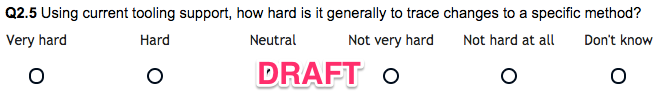
\includegraphics[width=0.98\columnwidth]{figures/example_likert_question}
  \caption{Example likert-scale question}
  \label{fig:example_likert_question}
\end{figure}

\textbf{Part 1} was designed to convey a general picture in regard of RQ1-2. We tried to provide a gentle entry and asked for the recency and a description of the participant's last activity with source code history (RQ1). To investigate the structural granularity (first part of RQ2) we let participants rate how interested they are in history at different levels, e.g. \textit{file}, \textit{class/module}, \textit{field/variable}, \textit{method/function}, \textit{block}. In terms of the temporal granularity (second part of RQ2) we asked for a description on how far in the past they normally examine history and how they decide for this time span.

\textbf{Part 2} first provided a brief scenario in line with the one described in Section~\ref{sec:scenario_general}: a developer is faced with a pull request and wants to understand better what the code that was changed is actually doing. Using this scenario, we wanted to gain more information about whether developers use source code history for program understanding tasks and what information they are searching for (RQ1). We first asked participants how familiar this scenario appears to them and then for a description of how they would approach this problem. We then isolated the imaginary change to a change to a \textit{single method} and asked participants how they would identify changes in history that changed this method as an example of a semantic unit. We asked subsequently how well the participant's described strategy would cope with complex structural changes to this method (e.g. renaming, moving to a different file). Concluding Part 2, we asked how hard it is generally to trace changes to a method with current tooling support and for a description of what makes this hard or easy. Responses would provide us a clear picture on whether developers struggle with the tools they use for purposes as in the scenario (RQ3).

\textbf{Part 3} then moved on to a practical instance of the general scenario from Part 2 on Github\footnote{XXX}. We created a sample pull request\footnote{XXX} in our forked repository of the \textit{Checkstyle} project described in Section~\ref{sec:motivation} that changed a specific method. We provided a link to the associated file history\footnote{XXX} and asked participants to describe how they would identify commits in this history that changed the method of interest. While we expected that the challenge of this task would become visible from these descriptions we also asked directly how well existing tools support this task (RQ3). With this background, we moved towards RQ4 and let participants rate how useful a semantic history (i.e. history of this method only) would be in this scenario and how hard it would be to find the commit that really introduced the sample method (e.g. in the face of multiple refactoring operations).

Where Parts 1-3 of the survey investigated in the potentials of a semantic history tool with both general questions and a specific scenario, \textbf{Part 4} showed for the first time what the output of such a tool \textit{could} look like. We mocked an output for the scenario in Part 3, showing the respective commits and diffs that changed the method alongside detailed descriptions of the changes in natural language. To inform RQ4 and the feasibility of our approach further, we now asked for a rating on (a) how helpful this output would be for a better understanding of the method, (b) how hard it would be to retrieve this type of information manually and (c) how valuable a tool would be that could generate this output. Finally, we gave participants the option to express what other information could have been valuable that was not in our mocked result view.

\fg{I have a feeling that readers who haven't seen our survey will not yet get a good enough picture of it with this description. Maybe we could think about illustrating the sample scenarios and especially our mocked output somehow. But I'm not sure.} 

\subsection{Participants}
\label{sec:survey-participants}

% Q5.1-Q5.6: (questions on participants' backgrounds)

We recruited XXX professional developers from industry (XXX) and academia (XXX). Participants were selected and contacted individually from the authors' professional networks. For this survey, we traded a large pool of participants (e.g. with advertisement of anonymous links) in favor of certainty of participants' professional backgrounds in order to avoid misleading responses due to lack of experience. The majority of job titles (XXX\%) were \textit{software developer/engineer} or analogical terms. The remaining XXX\% were academic positions like \textit{PHD student}, \textit{researcher} or \textit{professor}. XXX\% had more than 4 years of programming experience (XXX\% > 10 years) and XXX\% had been professional software developers for more than 4 years (XXX\% > 10 years). XXX\% had used source code history for more than 4 years (XXX\% > 10 years). Figure~\ref{fig:popular_tools} shows our participants' most frequently used source code history tools. Other tools mentioned were specific IDE's and their add-ons with JetBrains IDEs (IntelliJ/PHPStorm/WebStorm) being most present, followed by VSCode and Eclipse. A few other tools (e.g. GitLens, GitKraken) were mentioned as well, but were not very common. In our view, the XXX responses convey an expressive and generalizale impression on developers' relationships with source code history.

\begin{figure}[t!]
  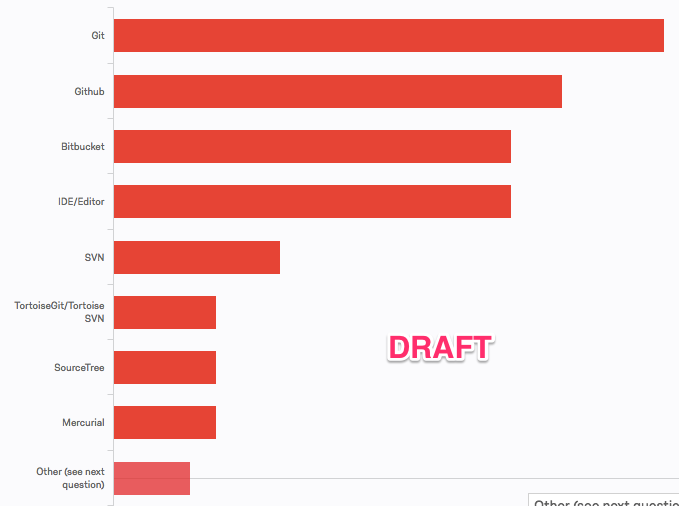
\includegraphics[width=0.98\columnwidth]{figures/popular_tools}
  \caption{Most popular source code history tools}
  \label{fig:popular_tools}
\end{figure}

\subsection{Survey Results}
\label{sec:survey-results}

We summarize and categorize the results of our survey in sequence of the research questions.

% ===================================================
% =================== RQ1 ===========================
% ===================================================

\mybox{\textbf{RQ1: }Do developers use source code history when they are working with code? If so, what are they trying to learn when they examine source code history?}

% Q1.1: How recently did you last use source code history of any kind?
% Q1.2: Please describe this most recent activity. How did you use source code history? What were you looking for? Did you find it? Did the tools you used support you in this investigation or could they be improved?

\noindent
The great majority of our participants use source code history very frequently: prior to the survey, XXX\% of participants had used source code history within two days prior to performing the survey (XXX\% < 1 week, XXX\% < one month). When asked for a description of this most recent activity, we first observe many common version control tasks, e.g. ``push some changes'', ``tagging the repo for a release'', ``merge branches'' or ``check what I modified''. We can also see many activities associated with accountability; participants checked ``who had been contributing'', ``who [they] could contact for dev support'' and ``who is associated with some changes''.

However, we can also deduce a big fraction of activities related to program understanding. Participants wanted to ``understand how the solution to a certain problem was implemented'' and ``how and why [a property] was changed''. Some participants were generally interested in the ``evolving of software architecture'' and in ``what steps a certain component took to get to the shape/position it was in''. The term \textit{understand} appeared XXX times when participants described their most recent activity.

Moreover, it becomes visible that developers search and navigate extensively through source code history to ``find reasons for [...] changes''. Participants ``browsed for a change made by a specific commit in the history'', ``[looked] for a specific change that might have introduced an issue'' and ``[looked] for an outdated implementation of a functionality''. They tried to ``[figure] out [a] history of changes'' and ``[compared] files over multiple commits''. The terms \textit{looked}, \textit{browsed}, \textit{searched} and \textit{navigated} appeared XXX times in the descriptions of most recent activities.

% Q2.1: Does this scenario sound familiar to you (i.e. have you encountered this in the past)?
% Q2.2: Please describe very briefly how you would approach this problem. What kinds of questions would you like to answer? What tools or approaches would you use to answer them?

When asked how familiar participants were with our scenario of a developer being faced with a pull request, not knowing what the code is actually doing, XXX\% replied with \textit{very familiar} or \textit{familiar}. When asked for a description of their strategy in this scenario, most participants replied that in a majority of cases their first step would be to approach the pull request author because ``they have to be accountable''. Other frequent strategies were to refer to issue trackers because they would tell ``what were the design decisions that lead to the change''. Other documentation from both within the pull request and external was also mentioned repeatedly, especially if the author is unavailable. Many developers would ``run that version locally and step through the different functions using a debugger'' because the pull request ``must contain a detailed setup to build an exact test environment''. Testing was another important topic and participants would be ``running the tests'' and inspect whether the change would ``cause any tests to change their fail/pass status''.

We can see that version history tools are another source of information and in fact the first step for some: ``my first step would be to look at the code history'' or ``fire up the history view [...] and hope for the best''. However, in comparison to other strategies (asking the author, documentation, tests, running changes locally), source code history would be used less frequently in this scenario\fg{because it's not good enough?!}.

% ===================================================
% =================== RQ2 ===========================
% ===================================================

\mybox{\textbf{RQ2: }In terms of their mental models and information needs, what level of structural and temporal granularity are most appropriate when using source code history?}

% Q1.3: In terms of source code granularity, how interested are you in gathering information on source code history at the following levels?

\noindent
Figure~\ref{fig:structural_granularity} shows how interested our participants were in gathering information on source code history at different levels of \textit{structural granularity}. We can see that developers are generally at least somewhat interested in all levels with the categories 'Neutral', 'Not very interested' and 'Not interested at all' having very low percentages. The most significant levels of interest were \textit{Method/Function} and \textit{Class/Module} with both having around XXX\% in the categories 'Very interested' and 'Interested'. This shows that developers are in fact mainly interested in the history of semantic code units rather than traditional, file- and text-based structural levels like \textit{File} or \textit{Directory/Package}, having only XXX\% and XXX\% in these categories respectively.

\begin{figure}[t!]
  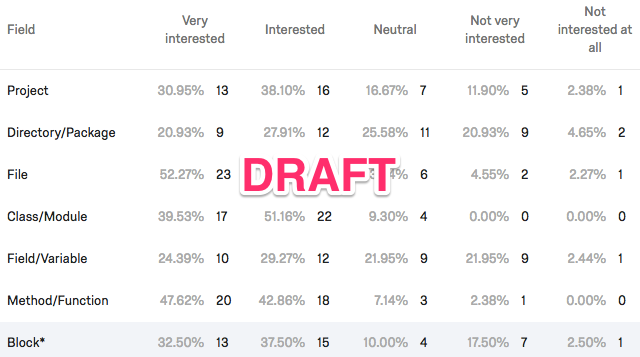
\includegraphics[width=0.98\columnwidth]{figures/structural_granularity}
  \caption{Structural granularity most appropriate when using source code history}
  \label{fig:structural_granularity}
\end{figure}

% Q1.4: When you use code history, how far in the past do you usually examine? How do you determine how far in the past you want to go?

To examine the \textit{temporal granularity} we asked participants how far in the past they usually examine and how they determine how far they want to go. The responses were mostly consistent in a way that ``this largely depends on the goal'' and that the time range can be very diverse because the fragment of interest is based on changes and commits rather than time. But there is also a clear thread that participants ``don't usually go [back] more than a few weeks'' or ``a couple of days'' in most cases, but at other times they ``look at the commit history years ago''. Interestingly, the cases where they examine further in the past seem to be related to program understanding tasks most often, e.g. when ``looking for the reason for a code change'', ``if some functionality seems odd or obsolete while reviewing source code'' or ``to understand why and how specific parts became the way they are today''.

% ===================================================
% =================== RQ3 ===========================
% ===================================================

\mybox{\textbf{RQ3: }How do developers identify the history of specific code units? How effectively does existing tooling support them?}

% Q2.3: Using source code history, how would you find changes to this method only? Please describe briefly.
% Q2.5: Using current tooling support, how hard is it generally to trace changes to a specific method?

\noindent
With the example code unit of a \textit{method} we referred back to our general pull request example and asked our participants how they would \textit{generally} identify the history of a method and how challenging this task is. We identified \textit{file history} as the most important strategy. Some participants described how they would limit the history to isolate changes to a method, e.g. using a combination of \texttt{git log} and \texttt{grep}. Many also mentioned recursive or iterative calls to \texttt{git blame} and more high-level sources of information like commit messages and issue trackers. To our surprise, only very few mentioned line- and range-based history, i.e. \texttt{git log -L} and higher-level abstractions like \textit{Show history for selection/method} in IntelliJ. Many participants immediately described this task as ``not trivial'', ``not easy'' and ``not the funniest job''  when asked for their strategy. Rating the difficulty of the task in a later question, XXX\% chose \textit{hard} or \textit{very hard}, XXX\% chose \textit{neutral}, and XXX\% chose \textit{not very hard} or \textit{not hard at all}.

% Q2.4: How well would your strategy cope with more complex structural changes, e.g. method renaming, moving of a method, refactoring?
% Q2.6: Given your answer to the previous question (Q2.5), what makes this hard or easy?

Figure~\ref{fig:strategy_complex_changes} shows participants' ratings of how well their strategies cope with more complex structural changes. It is visible that the change types \textit{method renames} and \textit{signature changes} are coped with quite well, but also that \textit{split into multiple methods} and especially \textit{move to different file} (XXX\% \textit{not very well} or \textit{not well at all}) are very hard to cope with. This is strongly confirmed by the responses to our question what would make this hard or easy where the main notion was that it depends on the complexity of changes: ``It's either easy (the method hasn't undergone complex changes) or challenging (the method has undergone complex changes). When it is challenging, it is VERY difficult.'' Many participants mentioned specifically that ``not knowing the semantics'' and the fact that ``[there] is no direct or explicit abstraction to method/class levels'' makes it very hard.

\begin{figure}[t!]
  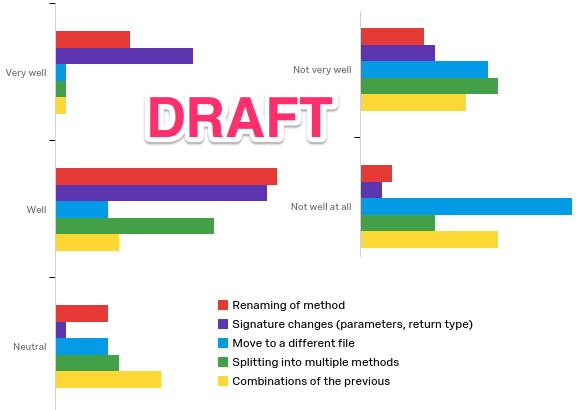
\includegraphics[width=0.98\columnwidth]{figures/strategy_complex_changes}
  \caption{How well do participants' strategies cope with more complex structural changes?}
  \label{fig:strategy_complex_changes}
\end{figure}

% Q3.1: In the above version history, how would you identify the commits in which the method of interest has changed? Please describe your strategy briefly.

When faced with our real-world example from the \textit{Checkstyle} repository \fg{I was just wondering here if it would be a lot better maybe if we could refer back to the example in the motivation. But it's not the example from the survey anymore. The example is better, but we're losing the connection to the survey a bit. Something to discuss.} and the associated file history, our participants assessed the task of identifying commits that changed the method as even more challenging than in the general previous questions. While some were quite plain that they can't think of a strategy for this scenario (``I have no idea how I would do this'', ``Not at all'', ``I sincerely have no idea''), we can see others who would come up with more advanced strategies like ``write a script'' or a ``divide and conquer mechanism'' but that this ``seems overkill''. But generally, we can see most participants falling back to the history of the file containing the method and they ``would dig through the history to find the method in each commit'' and ``open each one of them and manually inspect''. Some immediately pointed out the limits of this strategy: ``[if] the method comes from another class [...], that would be more difficult to trace'' and that ``it's annoying'', ``you got me with this one'', ``there's too much garbage noise'' and the ``revisions are too many to go through''. Some expressed unawareness of whether ``there is any tool that allows [them] to track the function across commits''.

% Q3.2: How well do existing tools support identifying these changes?
% Q3.4: How hard would it be to find the first commit for the given method and whether the method was really created then or if it was moved there from somewhere else (e.g. through a file renaming, or through a refactoring)?

When asked how well existing tools support identifying these changes, no participant said \textit{very well}, XXX\% said \textit{well} and XXX\% said \textit{neutral}. The great majority of participants rated with either \textit{not very well} or \textit{not well at all} (XXX\%). When asked how hard it would be to find the first commit that really introduced the method (rather than being just a refactoring commit), XXX\% replied with \textit{hard} or \textit{very hard}. 

% ===================================================
% =================== RQ4 ===========================
% ===================================================

\mybox{\textbf{RQ4: }Does augmenting history with semantic data improve program comprehension? How effectively can a semantic-aware code history viewer support program comprehension?}

% Q3.3: How useful would it be to have support for a more semantic history in this scenario (e.g. history for this method or class only)?
% Q4.1: Consider again the described situation of being faced with a pull request for a change of a method. How helpful would you consider the information above for getting a better understanding of the method and its history?
% Q4.2: How hard would you consider retrieving information on the history of a method with the above level of detail?
% Q4.3: If a tool could generate information in the fashion of the above on any method or other code unit, how valuable would you consider this tool?

\noindent
We mentioned previously that some participants mentioned that specifically the lack of semantic awareness of history tools makes it hard to trace the changes of methods (``not knowing the semantics''). When we now asked specifically how useful it would be to have support for a more semantic history for our example scenario  (i.e. history for this method only), XXX\% replied with \textit{very useful} or \textit{useful}. Participants were now faced with our mocked output of a fictitious semantic history tool, showing change descriptions and the commits and diffs that changed the method. When asked how valuable they would consider a tool generating this output automatically, XXX\% replied with \textit{very valuable} or \textit{valuable} and XXX\% consider retrieving this information manually \textit{hard} or \textit{very hard}. When asked how helpful they would consider this information for a better understanding of the method being faced with the pull request, XXX\% replied with \textit{very helpful} or \textit{helpful}. 

% Q4.4: What other information that is not in the descriptions above would you consider valuable?
% Q5.7: Do you have any final comments? Do you have any other ideas for tool support or systems to solve the general problems described in this survey and its scenarios? Is there anything else on your mind?

The generally positive attitute towards our idea was expressed explicitly by some when we asked for other information that could be valuable and in the final comments: ``having the information above would be a big improvement in the daily business'' and it would be great ``to generate a method-, class-, file-history/protocol in a human-readable way'' and to have ``version control that was method-aware, or aware of classes/modules''. As indicated before in RQ2, our \textit{method} example code unit was confirmed as ``definitely the best use case'' by some. However, some developers were ``not sure [they] would find rich method-level semantics that useful'' and to very few the usage of history for the described scenarios was overall unintuitive: ``why/how would I need/use history; to blame people for bugs?''. A few confirmed that ``the history of a [code unit] helps to understand a pull request, but [they] usually don't find the need to do so''. Some also expressed that ``it is not something I miss in my daily work but of course it would be very helpful in these rare situations where tracking [of code units] is needed''. Other responses also indicate that this more critical feedback - of history being not very useful for program understanding - may be ``because the tools that [they] use don't support this feature''. Some even thanked us that the survey helped them realized ``that [they] use VCS purely as an archive''.

We can deduce three main groups of other information that participants would find valuable that we did not present in our mocked semantic history outputs. First and foremost was \textit{authorship and intent}: developers seem to be highly interested in the question ``who made the changes and why''. While some commented that ``this is available in the linked commits so not really missing'', others regarded our output as just ``information when and what changed''. Along the same lines, many participants mentioned information from issue trackers associated with the changes being missing. Second was \textit{references}: many participants responded that ``it would be interesting to see where [a method]'s (been) used (in the past)'' and specifically ``the call reference to this method which in turn has been refracted just because of this method change''. Third was \textit{associated tests}: participants were interested in ``associated test runs/suites'' influenced by the change to the code unit because ``this would help to know if the methods were changed to fix specific bugs, or if they were refactored in an attempt to cleanup code''. We will discuss these suggestions more in Section~\ref{sec:discussion}.



%!TEX root = ../paper.tex

\section{Approach}
\label{sec:approach}

We implemented a prototype tool \textit{CodeShovel} for generating history summaries for Java and JavaScript methods in Git repositories. We chose \textit{method} as sample code unit because we assessed it as the most important level of abstraction. This was confirmed in our survey in Section~\ref{sec:survey}. We chose Git as version control system because it is by far the most prevalent in practice\cite{XXX}. In this section, we summarize our requirements and provide a brief overview of the core implementation. We shipped our prototype as a Bitbucket\footnote{XXX} add-on and we describe how we applied the core implementation to this specific version control tool.

\subsection{Requirements}
\label{sec:requirements}

From a high-level perspective, CodeShovel can be seen as a black box, taking a number of arguments describing a method in a repository as input and producing the method's history as output. The required inputs are as follows:

\begin{itemize}
	\item \textit{Repository}: path to a repository on the file system or URL to a remote repository.
	\item \textit{StartCommit}: hash of the commit to start from and move backwards through history.
	\item \textit{FilePath}: path of the file containing the method relative to the root folder of the repository.
	\item \textit{MethodName}: name of the target method.
	\item \textit{StartLine}: line number for the start of the method\footnote{There could be different methods with the same name, so this is required to identify the correct method. Files with multiple methods with the same name in the same line cannot be handled by CodeShovel at the moment (see Section~\ref{sec:future_work})}.
\end{itemize}

The output for one such input is the version history specific to this method, essentially as outlined in our Table~\ref{tbl:motivation:actual_history}, but with a natural language description of the changes made in each commit and additional meta-information. The additional information consists of simple commit data like the \textit{message}, \textit{author} and \textit{date}, enriched by more complex data like \textit{number of commits since the last commit that changed the method} (a) for the \textit{file} containing the method or (b) in the whole \textit{repository}. The actual output for our example in Table~\ref{tbl:motivation:actual_history} is shown in Figure~\ref{fig:sample_output}. In contrast to currently prevalent file- and line-range based history tools, this history does not show line range operations that did not actually change the method itself (a commonly found false positive in line-range based tools) but does include the moving of methods between files (a false negative in file-based tools). The latter effectively makes method histories produced by CodeStory much longer and richer than the prevalent tools because histories are not capped when refactoring operations occurred.

\begin{figure}[t!]
  
\includegraphics[width=0.98\columnwidth]{figures/sample_output}
  \caption{Actual output for our example in Section~\ref{sec:motivation}}
  \label{fig:sample_output}
\end{figure}

For our field study described in Section~\ref{sec:evaluation} and for general practicability, CodeShovel is integrated in a \textbf{BitBucket add-on}. It provides a user interface for selecting the method of interest and its environment, and an integrated view of the outputs.

\subsection{Implementation}
\label{sec:implementation}

We implemented CodeShovel in Java, mainly because it provided sufficiently capable AST parsers for both Java (\textit{JavaParser}\footnote{XXX}) and JavaScript (\textit{Nashorn}\footnote{XXX}) files. We used the Java Git interface \textit{JGit}\footnote{XXX} for Git operations (e.g. \texttt{git log}, \texttt{git checkout}) and for traversing commits in repositories. Given the required AST parsers in Java, the implementation is easily extensible for other languages: all core components with language-specific functionality were realized with abstract classes and interfaces and concrete language-specific implementations. Consequently, for adding other language 'adapters' the only requirement is an implementation of our interfaces. For example, our interface \texttt{Parser} defines a method signature \texttt{findMethodByNameAndLine(name, line)} which is implemented in our class \texttt{JavaParser} that knows how to find a method entity within a Java file, given its name and start line.

CodeShovel's core components are \textit{Parsers}, \textit{Tasks}, \textit{Interpreters} and \textit{Changes}:
\begin{itemize}
	\item \textit{Parsers}: responsible for AST parsing of language-specific files and extracting relevant components (e.g. methods).
	\item \textit{Tasks}: runtime environments for the execution of history tasks.
	\item \textit{Interpreters}: responsible for interpreting changes found for the target method in one specific commit compared to the previous.
	\item \textit{Changes}: entities representing commit-specific changes to the target method.
	\item \textit{Similarity Algorithms}: algorithms for matching methods in order to identify at what entry points a method history needs to be continued.
\end{itemize}

With these components, one \textbf{CodeShovel execution} with the inputs described in Section~\ref{sec:requirements} can be outlined as follows: a \textit{task} is created that saves the given inputs in its environment. Using \texttt{git log}, the history of the file containing the target method is created and for each commit the target method is identified using a \textit{similarity algorithm}. If the method cannot be identified, this is marked in the commit entity. The enriched file history is now iterated and the matched method of each commit is compared with the matched method of the previous commit using an \textit{in-file interpreter}. The result is one \textit{change} instance for each commit, according to the type hierarchy shown in Figure~\ref{fig:changes_hierarchy}. If no matched method can be found in the previous commit, the change type is \texttt{Introduced} and the \textit{task} is stopped at this point. Now, a \textit{cross-file interpreter} tries to find the method in other files that were changed in the commit using a \textit{similarity algorithm}. If it can find one, a new \textit{task} is created with the inputs being extracted from the identified method in the other file. The new task is executed in the same fashion as the previous one. This pattern is repeated recursively, until the \textit{cross-file interpreter} is unable to identify a method in a different file in the previous commits. In this case, the method was \textit{in fact} introduced in this commit and the recursive task chain will end and the resulting history is shown.

\begin{figure}[t!]
  
\includegraphics[width=0.98\columnwidth]{figures/changes_hierarchy}
  \caption{Type hierarchy of changes in CodeShovel}
  \label{fig:changes_hierarchy}
\end{figure}

Our \textbf{similarity algorithms} are currently based on five metrics that we assess to work for most programming languages:
\begin{itemize}
	\item \textit{Body similarity}: textual similarity\footnote{We use the Jaro–Winkler distance algorithm for determining textual similarity.} of the method body.
	\item \textit{Name similarity}: textual similarity of the method name.
	\item \textit{Parameter similarity}: textual similarity of parameter names and equality of parameter types (if supported by the language).
	\item \textit{Scope similarity}: name equality of the scope containing the method, e.g. the class or parent function (only used for in-file comparison).
	\item \textit{Line similiarity}: distance between the start line of the two methods (only used for in-file comparison).
\end{itemize}

Once all metrics are determined for a method pair, an overall similarity is created using weights for each metric. Currently, the weights are (XXX,XXX,XXX,XXX) for in-file comparison and (XXX,XXX) for cross-file comparison in sequence of the metrics in the list above. We have found these metrics and weights to be sufficiently accurate for our prototype implementation.

The integration of the core implementation in our \textbf{BitBucket add-on} was performed using the developer APIs provided by the \textit{Atlassian Plugin SDK}. Whenever a Java or JavaScript method is selected in the BitBucket Web application, a small popup with a link to the method history is shown. A \textit{Method History} view is then shown upon click which was implemented with the \textit{Servlet} component of the Atlassian Plugin SDK\footnote{XXX} (see Figure~\ref{fig:sample_output} for an example).

\begin{figure}[t!]
  
\includegraphics[width=0.98\columnwidth]{figures/bitbucket_popup}
  \caption{Popup with link to method history}
  \label{fig:bitbucket_popup}
\end{figure}


%!TEX root = ../paper.tex

\section{Evaluation}
\label{sec:evaluation}

\lipsum[1-10]
%!TEX root = ../devy.tex

\section{Discussion}
\label{sec:discussion}

\subsection{Interpretation of Results}
\label{sec:interpretation}

\lipsum[1-5]

\subsection{Threats to Validity}
\label{sec:threats}

\lipsum[1-3]

\subsection{Future Work}
\label{sec:future-work}

\lipsum[1-3]
%!TEX root=../devy.tex

\section{Related Work}
\label{sec:related-work}

\lipsum[1-5]
%!TEX root = ../devy.tex

\section{Conclusion}
\label{sec:conclusion}

\lipsum[1-4]

\pagebreak

\balance

% \cite{achi_2017_wachtel}
\bibliographystyle{ACM-Reference-Format}
\bibliography{paper}

\end{document}
